\documentclass[11pt]{article}
\usepackage[margin=1in]{geometry}
\usepackage[T1]{fontenc}
\usepackage[utf8]{inputenc}
\usepackage{lmodern}
\usepackage{microtype}
\usepackage{booktabs}
\usepackage{graphicx}
\usepackage{xcolor}
\usepackage{needspace}
\usepackage[colorlinks=true,linkcolor=blue!50!black,urlcolor=blue!50!black,citecolor=blue!50!black]{hyperref}

\title{A Benchmark of Kashmiri Proverbs in Nastaliq Script\\for Evaluating Large Language Models}
\author{Ahmed Bin Ajaz Bazaz\\
Independent Researcher, Srinagar, Jammu \& Kashmir, India\\
ORCID: \href{https://orcid.org/0009-0004-8298-3537}{0009-0004-8298-3537}\\
Source Code: \href{https://github.com/ahmed-ajaz17/Kashmiri-Proverb-Evaluation}{github.com/ahmed-ajaz17/Kashmiri-Proverb-Evaluation}\\
\texttt{ahmed.ajaz1408@gmail.com}}
\date{}

\begin{document}
\maketitle

\begin{abstract}
Kashmiri is a low-resource Indo-Aryan language written mainly in the Perso-Arabic (Nastaliq) script, and it is almost absent from language-model benchmarks. We present what is, to our knowledge, the first benchmark of Kashmiri proverbs in Nastaliq script. It contains 120 proverbs drawn from the public-domain collection of Knowles (1885), each with a Nastaliq form, a transliteration, an English meaning and its idiomatic context. We use the benchmark to test proverb understanding in six large language models through a four-option multiple-choice task, presenting each proverb in Nastaliq and in Roman transliteration. One model, Gemini 3.5 Flash, scores about 95\% in both scripts. The other five score between 40\% and 56\%, where chance is 25\%. Differences between scripts are small. Our results are limited by the size of the set, a single historical source, a single annotator, and possible training-data contamination. We release data, code and results openly.
\end{abstract}

\section{Introduction}
Proverbs compress cultural knowledge, metaphor and social norms into short fixed phrases. Understanding them requires more than word-level translation, so they are a useful probe of whether a language model knows a language and its culture, not just its vocabulary. Multilingual proverb benchmarks exist for a handful of high-resource languages \cite{liu2024maps}, but we are not aware of any for Kashmiri.

Kashmiri has several million speakers, mostly in the Kashmir Valley, and is written in a Perso-Arabic script commonly set in Nastaliq style. It is also written in Devanagari and Roman forms. Digital resources are scarce, and the Nastaliq form in particular is rarely seen in web-scale text corpora. Kashmiri is covered by large multilingual translation efforts such as NLLB \cite{nllb2022} and IndicTrans2 \cite{gala2023indictrans2}, which include it in Perso-Arabic script, but to our knowledge no benchmark tests cultural or figurative understanding in it.

This paper makes three contributions:
\begin{enumerate}
\item A dataset of 120 Kashmiri proverbs in Nastaliq with transliteration, English meaning and idiomatic context.
\item A multiple-choice evaluation protocol with a strict answer parser, run in two scripts (Nastaliq and Roman transliteration).
\item Results for six language models, with confidence intervals and an account of the limits of the evidence.
\end{enumerate}

\section{Related Work}
\paragraph{Proverb understanding.} Liu et al.\ \cite{liu2024maps} build a multilingual proverb benchmark (MAPS) covering six languages and show that language models handle figurative proverb meaning unevenly across languages. Our work follows the same idea for a language they do not cover.
\paragraph{Kashmiri in NLP.} NLLB \cite{nllb2022} and IndicTrans2 \cite{gala2023indictrans2} add Kashmiri to machine translation, which tests translation quality but not proverb or cultural understanding.

\section{Dataset}
\paragraph{Source.} Proverbs were selected from J.~Hinton Knowles, \emph{A Dictionary of Kashmiri Proverbs and Sayings} (1885) \cite{knowles1885}. The work is in the public domain. The Nastaliq text, English meanings and idiomatic context in our dataset were written by the author; the book itself does not provide them in this form.

\paragraph{Fields.} Each of the 120 entries has an identifier, the proverb in Nastaliq, a Roman transliteration, an English meaning and a note on the idiomatic context. The Roman transliteration keeps diacritics (for example \'a, \'u, \v{e}, \=a) and is adapted from the romanization used by Knowles; it is not a standardized phonetic scheme. Diacritics may be tokenized differently from plain ASCII, so the Roman results should be read with that in mind.

\paragraph{Text preparation.} The Nastaliq text was prepared by the author. Independent review by other native speakers is welcome, and corrections can be submitted through the project repository.

\paragraph{Licence.} Code is released under the MIT licence. We suggest CC BY 4.0 for the data.

\section{Method}
\paragraph{Task.} For each proverb the model sees a multiple-choice question with four options and must reply with one letter (A--D). One option is the correct meaning; the three distractors are the meanings of other proverbs in the dataset, sampled with a fixed random seed (42). Because the distractors are real meanings, they are fluent and plausible. The random baseline is 25\%.

\paragraph{Scripts.} Every proverb is tested twice: once shown in Nastaliq, once shown in Roman transliteration. The options are in English in both cases.

\paragraph{Models.} We tested Gemini 3.5 Flash, Gemini 3.5 Flash-Lite, Claude Haiku (\texttt{anthropic/claude-haiku-5.5}), DeepSeek (\texttt{deepseek/deepseek-v4.1-flash}), Qwen (\texttt{qwen/qwen3.8-27b}) and gpt-oss-120b (\texttt{openai/gpt-oss-120b}, via Groq). All were queried through their provider APIs at temperature 0 in November 2026.

\paragraph{Reasoning settings.} Models differ in how much they reason before answering. Gemini 3.5 Flash was run with its default thinking; several other models were run with reasoning set to low or off to keep replies short and within budget. This is a confound, and the results should not be read as a ranking of the underlying models.

\paragraph{Prompt.} All models received the same prompt, with the proverb shown in Nastaliq or in Roman transliteration:
\begin{quote}\small\ttfamily
The following is a Kashmiri proverb.\\[2pt]
Proverb: \{proverb\}\\[2pt]
Which option best gives the meaning of this proverb?\\
A. \{option A\}\\
B. \{option B\}\\
C. \{option C\}\\
D. \{option D\}\\[2pt]
Reply with only one letter: A, B, C or D.
\end{quote}
The final line, instructing a single-letter reply, is the same for every model; the format failures described below occurred despite it.

\paragraph{Answer parsing.} A reply counts only if it contains a clear final letter: a bare letter, ``Answer: X'', or a single bold letter near the end. Rambling or ambiguous replies count as no answer and are scored wrong; we never guess a letter. For Flash-Lite we also report a variant in which the model is asked for one follow-up (``what is your final answer?'') when its first reply has no clear letter, and a letter-only variant in which the API restricts the reply to A, B, C or D. Main results score the \emph{first reply only}.

\paragraph{Statistics.} We report accuracy with 95\% Wilson confidence intervals. We use the Wilson score interval \cite{wilson1927}. With $n=120$ each interval is roughly $\pm 9$ percentage points.

\section{Results}
Table~\ref{tab:main} and Figure~\ref{fig:main} show accuracy by model and script.

\begin{figure}[!ht]
\centering
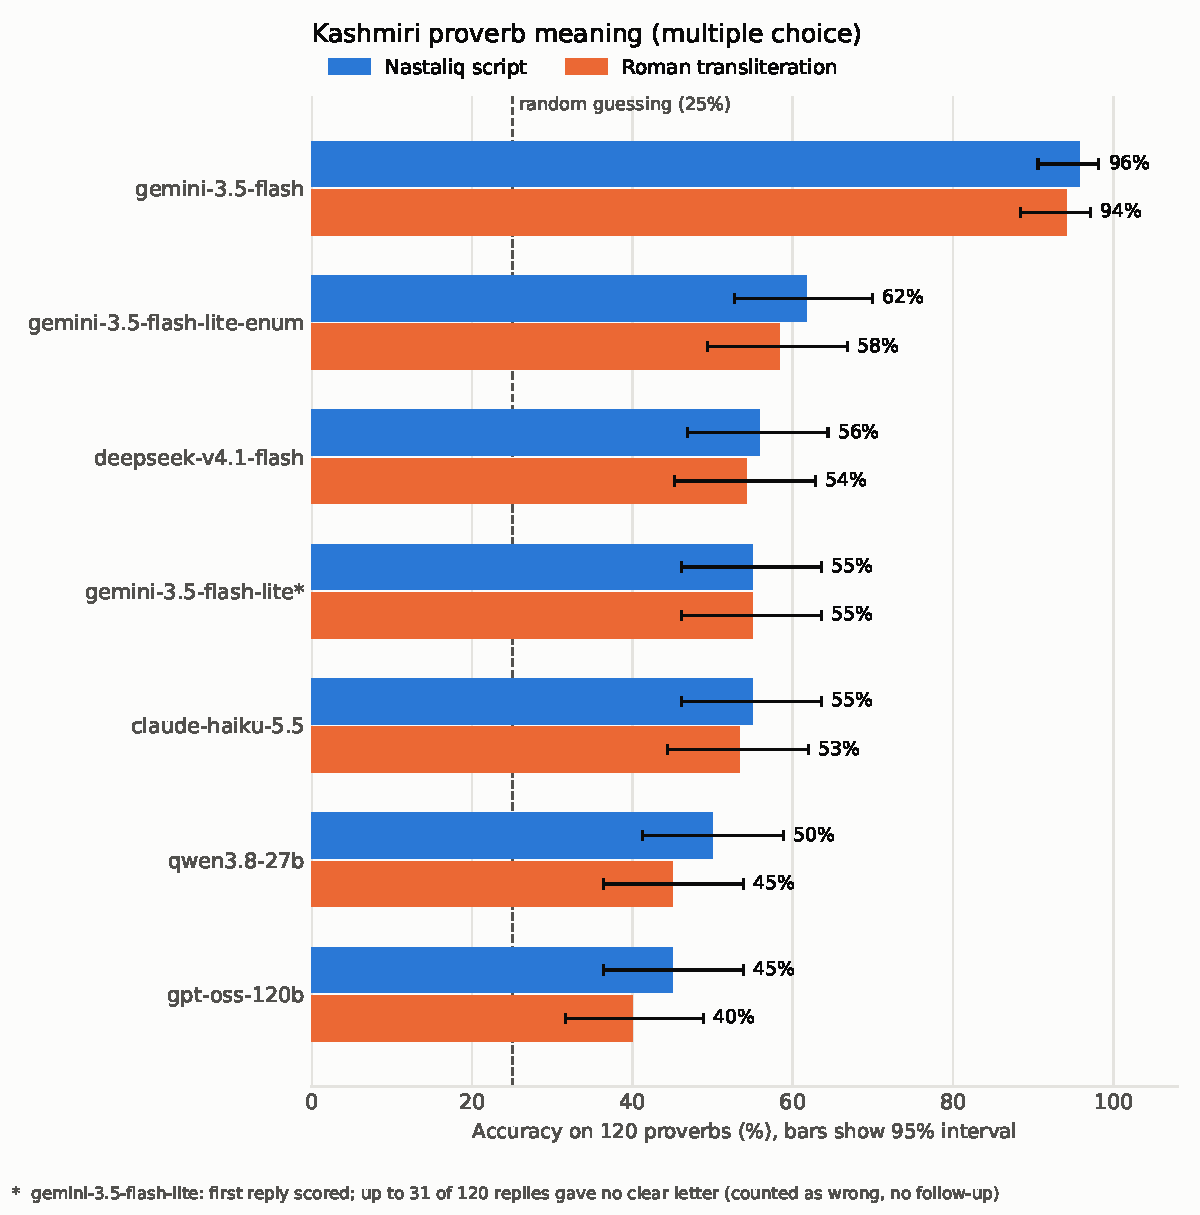
\includegraphics[width=0.9\linewidth]{figure_mcq.pdf}
\caption{Accuracy by model and script with 95\% confidence intervals. The dashed line marks chance (25\%). The chart also includes the constrained-decoding variant (\texttt{gemini-3.5-flash-lite-enum}), in which the API only allows the reply A, B, C or D; it is not in Table~\ref{tab:main}. The footnote in the chart notes the Flash-Lite replies that needed a follow-up question.}
\label{fig:main}
\end{figure}


\begin{table}[t]
\centering
\caption{Multiple-choice accuracy (\%) on 120 proverbs, first reply scored, with 95\% Wilson confidence intervals. Chance is 25\%.}
\label{tab:main}
\small
\begin{tabular}{lcc}
\toprule
Model & Nastaliq & Roman \\
\midrule
Gemini 3.5 Flash & 95.8 [90.6, 98.2] & 94.2 [88.4, 97.1] \\
DeepSeek (\texttt{deepseek/deepseek-v4.1-flash}) & 55.8 [46.9, 64.4] & 54.2 [45.3, 62.8] \\
Gemini 3.5 Flash-Lite & 55.0 [46.1, 63.6] & 55.0 [46.1, 63.6] \\
Claude Haiku & 55.0 [46.1, 63.6] & 53.3 [44.4, 62.0] \\
Qwen (\texttt{qwen/qwen3.8-27b}) & 50.0 [41.2, 58.8] & 45.0 [36.4, 53.9] \\
gpt-oss-120b & 45.0 [36.4, 53.9] & 40.0 [31.7, 48.9] \\
\bottomrule
\end{tabular}
\end{table}


\paragraph{Main findings.}
\begin{itemize}
\item Gemini 3.5 Flash is far ahead of the other models (about 95\% in both scripts). Its confidence interval does not overlap with any other model.
\item The other five models sit between 40\% and 56\%. All are well above chance, but the intervals overlap heavily, so we do not claim an ordering among them.
\item Differences between Nastaliq and Roman are small, at most five points, and inside the confidence intervals. We cannot say either script is easier.
\item Flash-Lite often failed to give a clear letter on its first reply (31 of 120 in Nastaliq, 19 of 120 in Roman). With a follow-up question its Nastaliq accuracy rises from 55.0\% to 65.8\%, which shows that part of the gap comes from answer formatting, not understanding alone.
\end{itemize}

\section{Limitations}
\begin{itemize}
\item \textbf{Small set from one source.} 120 proverbs from one 1885 collection cover limited vocabulary and dialect, and the language is dated.
\item \textbf{Possible contamination.} Knowles (1885) is available online and may be in the training data of some models. This could inflate scores, and may partly explain Gemini 3.5 Flash's high result. We have not tested for it.
\item \textbf{Single annotator.} The Nastaliq text and meanings were prepared by one person and have not yet been independently reviewed, so spelling variants or errors may remain.
\item \textbf{Unequal settings.} Reasoning effort and token limits differ between models, so the comparison is not controlled.
\item \textbf{Multiple choice only.} Distractors come from other proverbs and may be easier to rule out than an open-ended explanation. Models could use elimination without understanding the proverb.
\item \textbf{Single run.} Each condition was run once at temperature 0.
\end{itemize}

\Needspace{6\baselineskip}
\section{Conclusion and Future Work}
We introduced a small benchmark of Kashmiri proverbs in Nastaliq and found that one model handles it well while five others do only moderately better than chance. Natural next steps are independent review of the Nastaliq by additional native speakers, an open-ended explanation task scored by a judge model and by humans, a contamination check, a larger and more varied set of proverbs, and controlled reasoning settings across models.

\section*{Data and Code Availability}
Dataset, evaluation scripts and raw results are archived on Zenodo (\href{https://doi.org/10.5281/zenodo.24169347}{doi:10.5281/zenodo.24169347}) and available at the project repository: \href{https://github.com/ahmed-ajaz17/Kashmiri-Proverb-Evaluation}{github.com/ahmed-ajaz17/Kashmiri-Proverb-Evaluation}.

\begin{thebibliography}{9}
\bibitem{liu2024maps} C.~C.~Liu, F.~Koto, T.~Baldwin and I.~Gurevych. Are Multilingual LLMs Culturally-Diverse Reasoners? An Investigation into Multicultural Proverbs and Sayings. In \emph{Proceedings of NAACL}, 2024. arXiv:2309.08591.
\bibitem{nllb2022} NLLB Team, M.~R.~Costa-juss\`a et al. No Language Left Behind: Scaling Human-Centered Machine Translation. arXiv:2207.04672, 2022.
\bibitem{gala2023indictrans2} J.~Gala et al. IndicTrans2: Towards High-Quality and Accessible Machine Translation Models for all 22 Scheduled Indian Languages. \emph{Transactions on Machine Learning Research}, 2023. arXiv:2305.16307.
\bibitem{wilson1927} E.~B.~Wilson. Probable inference, the law of succession, and statistical inference. \emph{Journal of the American Statistical Association}, 22(158):209--212, 1927.
\bibitem{knowles1885} J.~Hinton Knowles. \emph{A Dictionary of Kashmiri Proverbs and Sayings}. Bombay: Education Society's Press, 1885.
\end{thebibliography}

\end{document}
